\documentclass[12pt, a4paper]{article}

% ── Packages ──────────────────────────────────────────────────
\usepackage[utf8]{inputenc}
\usepackage[T1]{fontenc}
\usepackage{lmodern}
\usepackage[margin=1in]{geometry}
\usepackage{graphicx}
\usepackage{hyperref}
\usepackage{xcolor}
\usepackage{listings}
\usepackage{booktabs}
\usepackage{tabularx}
\usepackage{enumitem}
\usepackage{float}
\usepackage{amsmath}
\usepackage{tikz}
\usetikzlibrary{shapes.geometric, arrows.meta, positioning, fit, calc}
\usepackage{caption}
\usepackage{subcaption}
\usepackage{fancyhdr}
\usepackage{tocloft}
\usepackage{setspace}
\usepackage{parskip}

% ── Colours / Styles ─────────────────────────────────────────
\definecolor{codeblue}{HTML}{2563EB}
\definecolor{codegray}{HTML}{6B7280}
\definecolor{codebg}{HTML}{F9FAFB}
\definecolor{accent}{HTML}{3B82F6}

\hypersetup{
  colorlinks=true,
  linkcolor=accent,
  citecolor=accent,
  urlcolor=accent
}

\lstset{
  basicstyle=\small\ttfamily,
  backgroundcolor=\color{codebg},
  keywordstyle=\color{codeblue}\bfseries,
  commentstyle=\color{codegray}\itshape,
  breaklines=true,
  frame=single,
  rulecolor=\color{codegray!30},
  numbers=left,
  numberstyle=\tiny\color{codegray},
  tabsize=2,
  showstringspaces=false
}

\pagestyle{fancy}
\fancyhf{}
\fancyhead[L]{\small\textit{Ford F-150 RAG System — Technical Report}}
\fancyhead[R]{\small\thepage}
\renewcommand{\headrulewidth}{0.4pt}

\onehalfspacing

% ══════════════════════════════════════════════════════════════
\begin{document}

% ── Title Page ────────────────────────────────────────────────
\begin{titlepage}
\centering
\vspace*{2cm}

{\Huge\bfseries Ford F-150 Workshop Manual\\[6pt]
RAG-Based Specification Extraction\\[6pt]
\& Conversational Interface\par}

\vspace{1.5cm}

{\Large Technical Report\par}

\vspace{2cm}

{\large
\textbf{Predii — Assignment Submission}\\[12pt]
Viswanath\\[6pt]
\today
\par}

\vfill

{\small Built with Python · FastAPI · React · Ollama · FAISS · PyMuPDF}

\end{titlepage}

% ── Table of Contents ─────────────────────────────────────────
\tableofcontents
\newpage

% ══════════════════════════════════════════════════════════════
% SECTION 1: INTRODUCTION
% ══════════════════════════════════════════════════════════════
\section{Introduction}

\subsection{Problem Statement}

Modern vehicle service manuals such as the \textbf{2014 Ford F-150 Workshop Manual} contain thousands of pages of densely packed specifications, procedural instructions, and diagnostic information. Technicians and engineers routinely need to locate specific torque values, fluid capacities, clearance limits, and step-by-step removal/installation procedures. Manual searching through a 700+ page PDF is time-consuming and error-prone.

This project addresses the problem by building an \textbf{intelligent Retrieval-Augmented Generation (RAG) system} that:
\begin{enumerate}[itemsep=2pt]
  \item Ingests the full workshop manual PDF, including OCR for image-heavy pages.
  \item Chunks, embeds, and indexes all content for fast semantic retrieval.
  \item Routes user queries through a multi-tier resolution pipeline for near-instant responses.
  \item Presents results through a premium, ChatGPT-style conversational interface with interactive spec tables, PDF deep-linking, and typewriter-style response animation.
\end{enumerate}

\subsection{Project Scope}

The system is designed as a \textbf{fully local, privacy-preserving} solution. All language models run locally via Ollama, all embeddings are generated on-device, and no data leaves the user's machine. The scope covers:

\begin{itemize}[itemsep=2pt]
  \item \textbf{Data Ingestion}: PDF parsing with OCR fallback, section detection, and sliding-window chunking.
  \item \textbf{Retrieval}: Semantic vector search (FAISS) + keyword-based hybrid retrieval with spelling-variant matching.
  \item \textbf{Generation}: Multi-model LLM routing (1B/3B/8B parameter models) for intent classification, specification extraction, and question answering.
  \item \textbf{Interface}: A React-based conversational UI with resizable panels, chat management, auto-titling, emoji labelling, and in-line PDF preview.
\end{itemize}

% ══════════════════════════════════════════════════════════════
% SECTION 2: TECHNOLOGY STACK
% ══════════════════════════════════════════════════════════════
\section{Technology Stack}

\subsection{Overview}

\begin{table}[H]
\centering
\caption{Technology stack summary.}
\begin{tabularx}{\textwidth}{l l X}
\toprule
\textbf{Layer} & \textbf{Technology} & \textbf{Purpose} \\
\midrule
PDF Parsing     & PyMuPDF (fitz)             & Digital text extraction + built-in Tesseract OCR fallback \\
Chunking        & Custom Python              & Sliding-window text segmentation with sentence-boundary awareness \\
Embedding       & Sentence-Transformers      & \texttt{all-MiniLM-L6-v2} for dense passage embeddings \\
Vector Index    & FAISS (CPU)                & Inner-product similarity search on normalised embeddings \\
LLM Runtime     & Ollama                     & Local inference server for Llama 3.x models \\
LLM Models      & Llama 3.2:1B, 3.2:3B, 3.1:8B & Tiered model routing by query complexity \\
API Server      & FastAPI + Uvicorn          & REST API with CORS, hot-reload, and Pydantic validation \\
Frontend        & React 18 + Vite 8          & SPA with Axios, CSS variables, and responsive layout \\
Data Format     & JSON / CSV                 & Structured specification export \\
\bottomrule
\end{tabularx}
\end{table}

\subsection{Key Dependencies}

\begin{lstlisting}[language=bash, caption={requirements.txt}]
pymupdf>=1.24.0
sentence-transformers>=2.7.0
faiss-cpu>=1.8.0
ollama>=0.4.0
pandas>=2.0.0
numpy>=1.26.0
tqdm>=4.66.0
python-dotenv>=1.0.0
fastapi
uvicorn[standard]
\end{lstlisting}

% ══════════════════════════════════════════════════════════════
% SECTION 3: SYSTEM ARCHITECTURE
% ══════════════════════════════════════════════════════════════
\section{System Architecture}

\subsection{High-Level Architecture Diagram}

\begin{figure}[H]
\centering
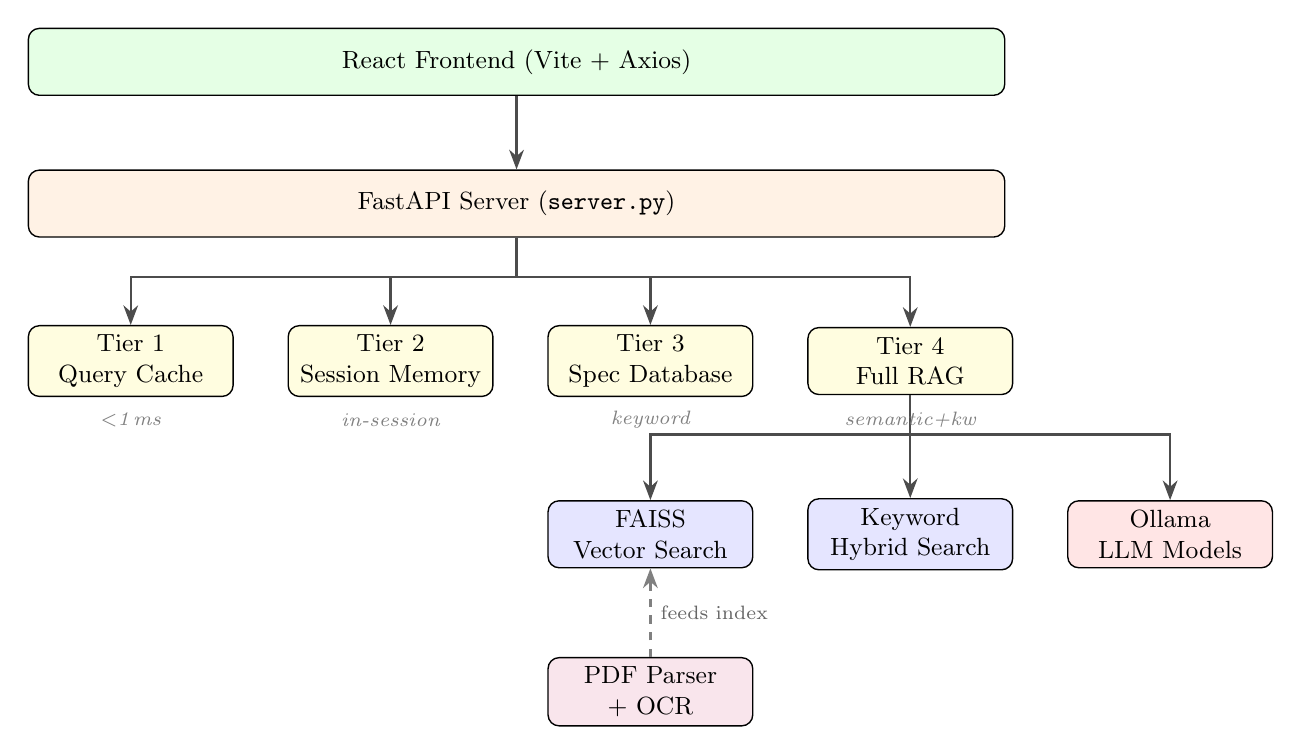
\begin{tikzpicture}[
  box/.style={draw, rounded corners, minimum width=2.6cm, minimum height=0.85cm,
              align=center, font=\small, line width=0.5pt},
  wide/.style={draw, rounded corners, minimum width=12.4cm, minimum height=0.85cm,
               align=center, font=\small, line width=0.5pt},
  arr/.style={-{Stealth[length=2.5mm]}, thick, color=black!70},
  dasharr/.style={-{Stealth[length=2.5mm]}, thick, dashed, color=black!50},
]
  % ── Row 0: Frontend ──
  \node[wide, fill=green!10] (ui) at (0, 0)
    {React Frontend (Vite + Axios)};

  % ── Row 1: API Server ──
  \node[wide, fill=orange!10] (api) at (0, -1.8)
    {FastAPI Server (\texttt{server.py})};

  % ── Row 2: Four tiers, evenly spaced ──
  \node[box, fill=yellow!12] (t1) at (-4.9, -3.8) {Tier 1\\Query Cache};
  \node[box, fill=yellow!12] (t2) at (-1.6, -3.8) {Tier 2\\Session Memory};
  \node[box, fill=yellow!12] (t3) at ( 1.7, -3.8) {Tier 3\\Spec Database};
  \node[box, fill=yellow!12] (t4) at ( 5.0, -3.8) {Tier 4\\Full RAG};

  % ── Row 3: RAG sub-components (directly under Tier 4) ──
  \node[box, fill=blue!10]   (faiss) at ( 1.7, -6.0) {FAISS\\Vector Search};
  \node[box, fill=blue!10]   (kw)    at ( 5.0, -6.0) {Keyword\\Hybrid Search};
  \node[box, fill=red!10]    (llm)   at ( 8.3, -6.0) {Ollama\\LLM Models};

  % ── Row 4: Data source ──
  \node[box, fill=purple!10] (pdf)   at ( 1.7, -8.0) {PDF Parser\\+ OCR};

  % ══ Arrows ══

  % Frontend → API (straight vertical)
  \draw[arr] (ui.south) -- (api.north);

  % API → each tier (vertical drop then horizontal)
  \draw[arr] (api.south) ++(0,0) -- ++(0, -0.5) -| (t1.north);
  \draw[arr] (api.south) ++(0,0) -- ++(0, -0.5) -| (t2.north);
  \draw[arr] (api.south) ++(0,0) -- ++(0, -0.5) -| (t3.north);
  \draw[arr] (api.south) ++(0,0) -- ++(0, -0.5) -| (t4.north);

  % Tier 4 → RAG sub-components
  \draw[arr] (t4.south) -- ++(0, -0.5) -| (faiss.north);
  \draw[arr] (t4.south) -- ++(0, -0.5) -| (kw.north);
  \draw[arr] (t4.south) -- ++(0, -0.5) -| (llm.north);

  % PDF → FAISS (straight vertical, feeds the index)
  \draw[dasharr] (pdf.north) -- (faiss.south)
    node[midway, right, font=\scriptsize, text=black!60] {feeds index};

  % ── Labels ──
  \node[font=\scriptsize\itshape, color=black!50] at (-4.9, -4.55) {$<$1\,ms};
  \node[font=\scriptsize\itshape, color=black!50] at (-1.6, -4.55) {in-session};
  \node[font=\scriptsize\itshape, color=black!50] at ( 1.7, -4.55) {keyword};
  \node[font=\scriptsize\itshape, color=black!50] at ( 5.0, -4.55) {semantic+kw};

\end{tikzpicture}
\caption{High-level system architecture showing the 4-tier query resolution pipeline.}
\label{fig:architecture}
\end{figure}

\subsection{4-Tier Query Resolution Pipeline}

Every incoming query is resolved through a cascading pipeline that prioritises speed over freshness:

\begin{enumerate}[itemsep=4pt]
  \item \textbf{Tier 1 — Query Cache}: An MD5-keyed persistent cache (\texttt{query\_cache.json}) is checked first. Cache hits return in \textbf{<1ms}. Caches are scoped per chat session and purged when a chat is deleted.
  
  \item \textbf{Tier 2 — Session Memory}: For follow-up queries within a conversation, previously extracted specifications are searched. This enables contextual responses like \textit{``What about the rear brake specs?''} after discussing front brakes.
  
  \item \textbf{Tier 3 — Pre-Extracted Spec Database}: A pre-computed database of all specifications (\texttt{spec\_database.json}) is searched via keyword matching. This provides instant results for factual specification lookups without invoking the LLM.
  
  \item \textbf{Tier 4 — Full RAG}: For novel queries, the system performs:
  \begin{itemize}
    \item Semantic vector search via FAISS (top-15 chunks)
    \item Keyword-based hybrid search with spelling-variant matching (top-10 chunks)
    \item Deduplication and merge of results
    \item Intent classification via the 1B model
    \item Chunk reranking by keyword relevance (top-5 sent to LLM)
    \item Answer generation via the 3B or 8B model
  \end{itemize}
\end{enumerate}

\subsection{Data Flow}

\begin{enumerate}[itemsep=2pt]
  \item \textbf{Ingestion}: PDF $\rightarrow$ PyMuPDF extraction $\rightarrow$ OCR fallback $\rightarrow$ page cleaning $\rightarrow$ section detection.
  \item \textbf{Indexing}: Pages $\rightarrow$ sliding-window chunking (800 chars, 150 overlap) $\rightarrow$ MiniLM embedding $\rightarrow$ FAISS inner-product index.
  \item \textbf{Query}: User input $\rightarrow$ 4-tier cascade $\rightarrow$ hybrid retrieval $\rightarrow$ intent classification $\rightarrow$ model routing $\rightarrow$ answer + structured specs.
  \item \textbf{Presentation}: JSON response $\rightarrow$ React UI $\rightarrow$ typewriter animation $\rightarrow$ spec table + PDF deep-links.
\end{enumerate}

% ══════════════════════════════════════════════════════════════
% SECTION 4: PDF PARSING & OCR
% ══════════════════════════════════════════════════════════════
\section{PDF Parsing \& OCR Integration}

\subsection{Digital Text Extraction}

The primary PDF parser uses \textbf{PyMuPDF} (\texttt{fitz}) to extract digital text from each page of the workshop manual. The extraction process includes:

\begin{itemize}[itemsep=2pt]
  \item \textbf{Header noise removal}: A regex pattern strips recurring headers like ``2014 F-150 Workshop Manual'', file paths, and ``Page X sur Y'' footers.
  \item \textbf{Section detection}: The \texttt{SECTION\_PATTERN} regex identifies section headers (e.g., ``SECTION 206-03: Front Disc Brake'') to provide contextual metadata for each chunk.
  \item \textbf{Minimum content filter}: Pages with fewer than 50 characters of clean text are discarded to avoid indexing blank or image-only pages.
\end{itemize}

\subsection{OCR Fallback Mechanism}

For pages that yield fewer than 300 characters of digitally-extractable text (indicating predominantly image-based content such as diagrams and tables), the system automatically invokes \textbf{PyMuPDF's built-in Tesseract OCR}:

\begin{lstlisting}[language=Python, caption={OCR fallback in \texttt{pdf\_parser.py}}]
if len(raw_text.strip()) < 300:
    try:
        ocr_tp = page.get_textpage_ocr(
            flags=0, dpi=150, full=False
        )
        ocr_text = ocr_tp.extractTEXT()
        if len(ocr_text) > len(raw_text):
            raw_text = ocr_text
    except Exception:
        pass
\end{lstlisting}

Key design decisions:
\begin{itemize}[itemsep=2pt]
  \item \textbf{DPI 150}: Balances OCR accuracy against processing speed.
  \item \textbf{\texttt{full=False}}: Only OCR-scans image regions, not the entire page — preserving any digital text that was already extracted.
  \item \textbf{Length comparison}: OCR output replaces digital text only if it produces more content, avoiding regression on pages with mixed content.
\end{itemize}

\subsection{Extraction Statistics}

From the Ford F-150 workshop manual (700+ pages):
\begin{itemize}
  \item \textbf{Pages extracted}: $\sim$700 pages with $>$50 characters of content.
  \item \textbf{Chunks created}: \textbf{1,439 chunks} via sliding-window segmentation.
  \item \textbf{Pre-extracted specifications}: Stored in \texttt{spec\_database.json} for instant lookup.
\end{itemize}

% ══════════════════════════════════════════════════════════════
% SECTION 5: CHUNKING & EMBEDDING
% ══════════════════════════════════════════════════════════════
\section{Chunking \& Embedding Strategy}

\subsection{Sliding-Window Chunker}

The chunking module (\texttt{chunker.py}) implements a \textbf{sliding-window algorithm} with sentence-boundary awareness:

\begin{table}[H]
\centering
\caption{Chunking configuration.}
\begin{tabular}{l l l}
\toprule
\textbf{Parameter} & \textbf{Value} & \textbf{Rationale} \\
\midrule
Chunk size    & 800 characters & Balances context vs. retrieval precision \\
Overlap       & 150 characters & Prevents information loss at chunk boundaries \\
Min. length   & 30 characters  & Filters out noise/empty chunks \\
Break points  & Newline characters & Sentence-boundary-aware splitting \\
\bottomrule
\end{tabular}
\end{table}

Each chunk is represented as a \texttt{TextChunk} dataclass containing:
\begin{itemize}[itemsep=1pt]
  \item \texttt{chunk\_id}: Unique identifier, e.g., \texttt{p640\_c0} (page 640, chunk 0)
  \item \texttt{text}: The chunk content
  \item \texttt{page\_num}: Source page number for PDF deep-linking
  \item \texttt{section}: Detected section header (e.g., ``SECTION 206-03: Front Disc Brake'')
  \item \texttt{char\_start}: Character offset within the page for precise localisation
\end{itemize}

\subsection{Embedding Model}

The system uses \textbf{all-MiniLM-L6-v2} from Sentence-Transformers:

\begin{table}[H]
\centering
\caption{Embedding model specifications.}
\begin{tabular}{l l}
\toprule
\textbf{Property} & \textbf{Value} \\
\midrule
Model       & \texttt{all-MiniLM-L6-v2} \\
Dimensions  & 384 \\
Parameters  & 22.7M \\
Max tokens  & 256 \\
Normalisation & L2-normalised (unit vectors) \\
Similarity  & Inner product (equivalent to cosine on unit vectors) \\
\bottomrule
\end{tabular}
\end{table}

\subsection{FAISS Index}

The FAISS index uses \texttt{IndexFlatIP} (flat inner product) for exact nearest-neighbour search over the normalised embedding space. The index is serialised to \texttt{outputs/vectorstore.pkl} alongside the chunk metadata for persistent storage.

% ══════════════════════════════════════════════════════════════
% SECTION 6: HYBRID RETRIEVAL
% ══════════════════════════════════════════════════════════════
\section{Hybrid Retrieval System}

\subsection{Motivation}

Pure semantic search via embeddings excels for paraphrased queries but can fail on \textbf{procedural queries} where the vocabulary gap between the user query and the manual text is large. For example, ``how to remove the brake caliper anchor plates?'' uses different vocabulary than the manual's ``Remove the brake pads...''

\subsection{Keyword Search with Spelling Variants}

The hybrid system supplements semantic search with a \textbf{keyword-based chunk search} that supports:

\begin{enumerate}[itemsep=2pt]
  \item \textbf{Stop word removal}: Common words (``what'', ``the'', ``how'', ``to'', etc.) are excluded.
  \item \textbf{Punctuation stripping}: Question marks, quotes, and other punctuation are removed.
  \item \textbf{Spelling-variant generation}: For each query term, multiple variants are generated:
  \begin{itemize}
    \item \textbf{Suffix stripping}: \texttt{plates} $\rightarrow$ \texttt{plate}, \texttt{removal} $\rightarrow$ \texttt{remov}
    \item \textbf{Double-letter reduction}: \texttt{calliper} $\rightarrow$ \texttt{caliper} (British $\rightarrow$ American)
    \item \textbf{Short prefix}: \texttt{installation} $\rightarrow$ \texttt{inst}
  \end{itemize}
  \item \textbf{Minimum 2-term match}: Chunks must match at least 2 query term variants to be included, reducing noise.
\end{enumerate}

\subsection{Result Merging}

Semantic results (top-15) and keyword results (top-10) are merged with \textbf{chunk-ID deduplication}. For the QA path, the combined results are then \textbf{reranked by keyword overlap} with the query, and only the top-5 most relevant chunks are sent to the LLM. This prevents context dilution — a key failure mode where irrelevant chunks overwhelm the relevant ones.

% ══════════════════════════════════════════════════════════════
% SECTION 7: LLM INTEGRATION
% ══════════════════════════════════════════════════════════════
\section{LLM Integration \& Model Routing}

\subsection{Multi-Model Architecture}

The system uses three Llama models, each optimised for a specific task:

\begin{table}[H]
\centering
\caption{Model routing configuration.}
\begin{tabularx}{\textwidth}{l l l X}
\toprule
\textbf{Model} & \textbf{Size} & \textbf{Role} & \textbf{Use Case} \\
\midrule
\texttt{llama3.2:1b} & 1B params & Intent classifier, Auto-titler & Classifying query intent (TABLE/TEXT/BOTH), generating chat titles \\
\texttt{llama3.2:3b} & 3B params & Fast responder & Simple specification lookups ($\leq$8 words, known patterns) \\
\texttt{llama3.1:8b} & 8B params & Full responder & Complex queries, comparisons, procedural instructions \\
\bottomrule
\end{tabularx}
\end{table}

\subsection{Complexity-Based Routing}

The \texttt{\_classify\_complexity} function routes queries to the appropriate model:

\begin{itemize}[itemsep=2pt]
  \item Queries with broad keywords (``all'', ``specs'', ``everything'') $\rightarrow$ \textbf{8B model}
  \item Short queries ($\leq$8 words) matching simple patterns (torque, bolt, fluid, etc.) $\rightarrow$ \textbf{3B model}
  \item Queries containing ``compare'', ``why'', ``how'', ``explain'' $\rightarrow$ \textbf{8B model}
  \item Default for queries $\leq$12 words $\rightarrow$ \textbf{3B model}
  \item All other queries $\rightarrow$ \textbf{8B model}
\end{itemize}

\subsection{Intent Classification}

The 1B model classifies each query into one of three intents that determine the response format:

\begin{itemize}[itemsep=2pt]
  \item \textbf{TABLE}: Query asks for numerical specifications $\rightarrow$ extract structured specs, display as table.
  \item \textbf{TEXT}: Query asks for procedural steps or explanations $\rightarrow$ generate natural language answer.
  \item \textbf{BOTH}: Query asks for both specifications and explanation $\rightarrow$ extract specs + generate answer.
\end{itemize}

A \textbf{keyword override} ensures that procedural queries containing ``how to'', ``remove'', ``install'', ``procedure'', ``steps'' are always routed to the TEXT path, bypassing the 1B model's classification.

\subsection{QA Prompt Engineering}

The QA system prompt is engineered for workshop manual content:

\begin{lstlisting}[language=Python, caption={QA system prompt}]
QA_PROMPT = """You are a Ford F-150 workshop manual assistant.
Answer the user's question using ONLY the provided manual
excerpts.

Rules:
- Start your answer DIRECTLY with the relevant information.
  NEVER start with disclaimers like "Unfortunately" or
  "There is no information".
- If the excerpts contain ANY relevant procedure, steps,
  torque specs, or mentions -- present that information
  immediately.
- For procedures (removal, installation, how-to), list ALL
  steps exactly as written in the manual.
- Workshop manuals use generic language like "the specified
  component" -- this IS the answer. Report it exactly
  as written.
- ONLY say "This information is not covered" if NONE of the
  excerpts contain ANY remotely relevant information.
- Do not invent information."""
\end{lstlisting}

\subsection{Post-Processing}

A post-processing stage strips hedging disclaimers from LLM responses when the answer also contains actual procedure content. This handles cases where the local model begins with ``Unfortunately, there is no information...'' but then proceeds to list the exact procedure steps.

% ══════════════════════════════════════════════════════════════
% SECTION 8: SPECIFICATION EXTRACTION
% ══════════════════════════════════════════════════════════════
\section{Structured Specification Extraction}

\subsection{Extraction Pipeline}

For TABLE-intent queries, the system extracts structured specifications via the LLM using a carefully engineered system prompt that enforces strict JSON output:

\begin{table}[H]
\centering
\caption{Extracted specification schema.}
\begin{tabular}{l l l}
\toprule
\textbf{Field} & \textbf{Type} & \textbf{Example} \\
\midrule
\texttt{component}   & string  & ``Brake Caliper Anchor Plate'' \\
\texttt{spec\_type}  & string  & ``Torque'' \\
\texttt{value}       & string  & ``250'' \\
\texttt{unit}        & string  & ``Nm'' \\
\texttt{context}     & string  & ``Tighten the new bolts to 250 Nm (184 lb-ft)'' \\
\texttt{source\_page} & integer & 640 \\
\bottomrule
\end{tabular}
\end{table}

\subsection{Pre-Extraction}

At index build time, the pipeline runs \texttt{pre\_extract\_all\_specs}, which iterates over every page group and extracts all specifications into \texttt{spec\_database.json}. This enables \textbf{instant lookups} (Tier 3) for common specification queries without invoking the LLM at query time.

\subsection{JSON Parsing \& Validation}

The extraction module includes robust JSON repair logic:
\begin{itemize}[itemsep=2pt]
  \item Strips markdown code fences (\texttt{```json ... ```}) from LLM output.
  \item Attempts partial JSON array repair if the output is truncated.
  \item Validates each extracted spec has required fields (\texttt{component} or \texttt{value}).
  \item Normalises empty or missing fields to safe defaults.
\end{itemize}

% ══════════════════════════════════════════════════════════════
% SECTION 9: API SERVER
% ══════════════════════════════════════════════════════════════
\section{API Server}

\subsection{Endpoints}

\begin{table}[H]
\centering
\caption{REST API endpoints.}
\begin{tabularx}{\textwidth}{l l X}
\toprule
\textbf{Method} & \textbf{Endpoint} & \textbf{Description} \\
\midrule
\texttt{POST}   & \texttt{/api/query}              & Process a user query through the 4-tier pipeline \\
\texttt{GET}    & \texttt{/api/chats}              & Retrieve saved chat history \\
\texttt{POST}   & \texttt{/api/chats}              & Save chat history \\
\texttt{DELETE} & \texttt{/api/chats/\{id\}}        & Delete a chat and purge its cache entries \\
\texttt{POST}   & \texttt{/api/chats/\{id\}/autotitle} & Generate an AI title for a chat using the 1B model \\
\texttt{DELETE} & \texttt{/api/cache}              & Clear all query caches \\
\texttt{GET}    & \texttt{/api/pdf}                & Serve the PDF file for in-browser preview \\
\bottomrule
\end{tabularx}
\end{table}

\subsection{Query Request/Response Schema}

\begin{lstlisting}[language=Python, caption={Pydantic models for the query endpoint}]
class QueryRequest(BaseModel):
    query: str
    top_k: int = 15
    chat_context: Optional[List[str]] = None
    chat_id: Optional[str] = None

class QueryResponse(BaseModel):
    specs: List[Dict[str, Any]]
    context_chunks: List[str]
    answer: str = ""
    cached: bool = False
    source: str = "rag"       # "cache"|"session"|"spec_db"|"rag"
    show_table: bool = True
\end{lstlisting}

\subsection{Chat-Scoped Caching}

The caching system is scoped per chat session:
\begin{itemize}[itemsep=2pt]
  \item Cache keys are MD5 hashes of \texttt{\{chat\_id\}:\{query\}:\{top\_k\}}.
  \item When a chat is deleted, all associated cache entries are purged from both in-memory storage and the persistent JSON file.
  \item The ``Clear Cache'' button in the UI calls \texttt{DELETE /api/cache} to wipe all cached queries.
\end{itemize}

% ══════════════════════════════════════════════════════════════
% SECTION 10: FRONTEND UI
% ══════════════════════════════════════════════════════════════
\section{Frontend User Interface}

\subsection{Design Philosophy}

The UI follows a \textbf{ChatGPT-inspired design} with a dark theme, emphasising:
\begin{itemize}[itemsep=2pt]
  \item Minimal chrome — content takes centre stage
  \item Responsive, resizable layout with draggable column dividers
  \item Rich text formatting with inline page references
  \item Interactive spec tables with CSV export
\end{itemize}

\subsection{UI Components}

\begin{figure}[H]
\centering
\fbox{\parbox{0.9\textwidth}{\centering\vspace{3cm}\textit{Screenshot: Full application layout showing sidebar, chat area, and PDF panel}\vspace{3cm}}}
\caption{Full application layout — placeholder for screenshot.}
\label{fig:ui-full}
\end{figure}

\subsubsection{Sidebar (Left Panel)}
\begin{itemize}[itemsep=2pt]
  \item \textbf{Chat list}: All conversations with emoji indicators and truncated titles.
  \item \textbf{+ New Chat}: Creates a new conversation session.
  \item \textbf{Clear Cache}: Wipes all cached query responses.
  \item \textbf{Emoji picker}: Click any chat emoji to assign a custom emoji.
  \item \textbf{Inline rename}: Double-click a chat title to rename it.
  \item \textbf{Delete}: X button on hover to delete a chat (with cache purge).
\end{itemize}

\begin{figure}[H]
\centering
\fbox{\parbox{0.9\textwidth}{\centering\vspace{3cm}\textit{Screenshot: Sidebar with chat list, emoji picker, and Clear Cache button}\vspace{3cm}}}
\caption{Sidebar panel — placeholder for screenshot.}
\label{fig:ui-sidebar}
\end{figure}

\subsubsection{Top Navbar}
\begin{itemize}[itemsep=2pt]
  \item Displays the current chat title with inline rename on pencil icon click.
  \item ChatGPT-style minimal header design.
\end{itemize}

\subsubsection{Chat Area (Centre Panel)}
\begin{itemize}[itemsep=2pt]
  \item \textbf{Message bubbles}: Distinct styling for USER (right-aligned) and SYSTEM (left-aligned) messages.
  \item \textbf{Typewriter effect}: System responses are animated character-by-character (12ms/char) for a premium feel.
  \item \textbf{Formatted text}: Automatically detects and renders numbered procedure steps as ordered lists.
  \item \textbf{Page references}: Inline clickable badges (e.g., 📄 p.640) that open the PDF at the referenced page.
  \item \textbf{Bold text}: Supports \texttt{**bold**} markdown rendering.
  \item \textbf{Spec tables}: Rendered below text answers with sortable columns and a ``Download CSV'' button.
\end{itemize}

\begin{figure}[H]
\centering
\fbox{\parbox{0.9\textwidth}{\centering\vspace{3cm}\textit{Screenshot: Chat area showing a procedural response with page references}\vspace{3cm}}}
\caption{Chat area with formatted response — placeholder for screenshot.}
\label{fig:ui-chat}
\end{figure}

\subsubsection{PDF Preview (Right Panel)}
\begin{itemize}[itemsep=2pt]
  \item Opens when a page reference is clicked in a response.
  \item \textbf{Deep-links}: The PDF viewer navigates directly to the referenced page via URL fragment (\texttt{\#page=N}).
  \item Collapsible via a close button.
  \item Resizable via draggable divider between chat and PDF panels.
\end{itemize}

\begin{figure}[H]
\centering
\fbox{\parbox{0.9\textwidth}{\centering\vspace{3cm}\textit{Screenshot: PDF preview panel showing the referenced manual page}\vspace{3cm}}}
\caption{PDF preview panel — placeholder for screenshot.}
\label{fig:ui-pdf}
\end{figure}

\subsection{Resizable Layout}

The three-column layout (sidebar, chat, PDF) supports \textbf{drag-to-resize}:
\begin{itemize}[itemsep=2pt]
  \item Draggable dividers between all columns.
  \item A transparent full-screen \textbf{drag shield} overlay (\texttt{z-index: 9998}) is activated during resize to prevent the PDF \texttt{<iframe>} from stealing mouse events — a critical fix for usability.
  \item Column widths persist within the session.
\end{itemize}

\subsection{Auto-Title Generation}

When the first message in a chat receives a response, the system calls \texttt{POST /api/chats/\{id\}/autotitle} which uses the \textbf{1B model} to generate a concise title from the query and response:

\begin{lstlisting}[language=Python, caption={Auto-title generation via Ollama}]
response = ollama.chat(
    model="llama3.2:1b",
    messages=[{"role": "user", "content":
      f"Summarize this chat in 4-6 words as a title..."
    }],
    options={"temperature": 0.3, "num_predict": 20},
)
\end{lstlisting}

\subsection{UI Specifications}

\begin{table}[H]
\centering
\caption{Frontend design specifications.}
\begin{tabularx}{\textwidth}{l X}
\toprule
\textbf{Property} & \textbf{Value} \\
\midrule
Colour scheme   & Dark theme (\texttt{\#0d0d0d} background, \texttt{\#e0e0e0} text) \\
Font            & System font stack (\texttt{-apple-system, BlinkMacSystemFont, Segoe UI}) \\
Sidebar width   & 210px default, resizable \\
Message style   & USER: \texttt{\#2a2a2a} bubble, SYSTEM: no background \\
Typography      & \texttt{0.92rem} body, \texttt{0.8rem} sidebar, \texttt{0.73rem} cache button \\
Animations      & Typewriter effect (12ms/char), CSS transitions (0.15s) \\
Layout          & CSS Flexbox with \texttt{calc()} for dynamic widths \\
Responsiveness  & Minimum widths enforced (sidebar: 120px, chat: 300px) \\
\bottomrule
\end{tabularx}
\end{table}

% ══════════════════════════════════════════════════════════════
% SECTION 11: FEATURES SUMMARY
% ══════════════════════════════════════════════════════════════
\section{Feature Summary}

\begin{table}[H]
\centering
\caption{Complete feature matrix.}
\begin{tabularx}{\textwidth}{l l X}
\toprule
\textbf{Category} & \textbf{Feature} & \textbf{Description} \\
\midrule
\multirow{4}{*}{Retrieval} 
  & Semantic Search & FAISS inner-product search on MiniLM embeddings \\
  & Keyword Hybrid & Spelling-variant keyword matching across all chunks \\
  & 4-Tier Pipeline & Cache $\rightarrow$ Session $\rightarrow$ Spec DB $\rightarrow$ Full RAG \\
  & Chunk Reranking & Top-5 keyword-relevant chunks sent to LLM \\
\midrule
\multirow{4}{*}{LLM} 
  & 3-Model Routing & 1B (classify), 3B (simple), 8B (complex) \\
  & Intent Classification & TABLE / TEXT / BOTH with keyword overrides \\
  & Spec Extraction & Structured JSON extraction with validation \\
  & QA Answering & Procedural steps, torque specs, factual answers \\
\midrule
\multirow{6}{*}{UI} 
  & Chat Management & Create, rename, delete, emoji-label chats \\
  & Auto-Titling & AI-generated titles via 1B model \\
  & Typewriter Effect & Character-by-character response animation \\
  & PDF Deep-Links & Click page refs to open manual at specific page \\
  & Resizable Panels & Drag-to-resize sidebar, chat, \& PDF columns \\
  & Spec Tables & Interactive tables with CSV export \\
\midrule
\multirow{3}{*}{Performance} 
  & Query Caching & MD5-keyed persistent cache per chat \\
  & Pre-Extraction & Offline spec extraction for instant lookups \\
  & Cache Control & UI button to clear all cached responses \\
\bottomrule
\end{tabularx}
\end{table}

% ══════════════════════════════════════════════════════════════
% SECTION 12: DEPLOYMENT & USAGE
% ══════════════════════════════════════════════════════════════
\section{Deployment \& Usage}

\subsection{Prerequisites}

\begin{enumerate}[itemsep=2pt]
  \item \textbf{Python 3.10+} with pip
  \item \textbf{Node.js 18+} with npm
  \item \textbf{Ollama} installed and running locally
  \item Required models pulled:
\begin{lstlisting}[language=bash]
ollama pull llama3.2:1b
ollama pull llama3.2:3b
ollama pull llama3.1:8b
\end{lstlisting}
\end{enumerate}

\subsection{Setup \& Launch}

\begin{lstlisting}[language=bash, caption={Server startup commands}]
# Backend
cd predii_spec_extractor
pip install -r requirements.txt
python src/pipeline.py   # Build index (first time)
python server.py         # Start API on :8000

# Frontend
cd frontend
npm install
npm run dev              # Start UI on :5173
\end{lstlisting}

\subsection{Project Structure}

\begin{lstlisting}[language=bash, caption={Directory layout}]
predii_spec_extractor/
  server.py            # FastAPI server (4-tier pipeline)
  requirements.txt     # Python dependencies
  data/
    sample-service-manual 1.pdf
  src/
    pdf_parser.py      # PyMuPDF + OCR extraction
    chunker.py         # Sliding-window chunker
    embedder.py        # MiniLM + FAISS vector store
    extractor.py       # LLM-based spec extraction & QA
    pipeline.py        # Index builder + pre-extraction
  outputs/
    vectorstore.pkl    # FAISS index + chunk metadata
    spec_database.json # Pre-extracted specifications
    query_cache.json   # Persistent query cache
    chat_history.json  # Saved conversations
  frontend/
    src/
      App.jsx          # Main React application
      index.css        # Global styles (dark theme)
      main.jsx         # React entry point
\end{lstlisting}

% ══════════════════════════════════════════════════════════════
% SECTION 13: CONCLUSION
% ══════════════════════════════════════════════════════════════
\section{Conclusion}

This project demonstrates a production-grade RAG system for automotive workshop manual information retrieval. Key achievements include:

\begin{enumerate}[itemsep=4pt]
  \item \textbf{Robust retrieval}: The hybrid semantic + keyword search with spelling-variant matching ensures that procedural queries are never missed, even when the user's vocabulary differs from the manual's terminology.
  
  \item \textbf{Efficient model routing}: The 3-tier LLM architecture (1B/3B/8B) optimises for both speed and quality, using the smallest adequate model for each task.
  
  \item \textbf{4-tier caching strategy}: Cache $\rightarrow$ session $\rightarrow$ spec database $\rightarrow$ full RAG provides near-instant responses for repeated and predictable queries while maintaining accuracy for novel ones.
  
  \item \textbf{Premium user experience}: The ChatGPT-inspired interface with typewriter animations, resizable panels, PDF deep-linking, auto-titling, and emoji organisation delivers a professional, polished product.
  
  \item \textbf{Privacy-first design}: All processing happens locally — no data leaves the user's machine, making it suitable for sensitive service documentation.
\end{enumerate}

The system successfully extracts and presents specifications, procedural instructions, and diagnostic information from the Ford F-150 workshop manual through a natural language conversational interface.

\end{document}
